\documentclass{article}
\usepackage[utf8]{inputenc}
\usepackage{xcolor}
\usepackage{graphicx}
\usepackage{float}
\usepackage{minted}
\usepackage{circuitikz}
\usepackage{tikz}
\usetikzlibrary{shapes, arrows, calc, positioning, circuits.logic.US, circuits.logic.IEC}
\usepackage{geometry}
\geometry{a4paper, margin=1in}
\usepackage{hyperref}
\usemintedstyle{trac}

\usepackage{fancyhdr}
\pagestyle{fancy}
\fancyhf{}
\renewcommand{\headrulewidth}{0pt}
\fancyfoot[C]{\small 010153101 Digital Circuit and Microprocessor Fundamental \\ Semester 2/2025}
\fancyfoot[R]{\thepage}

\fancypagestyle{plain}{%
  \fancyhf{}%
  \fancyfoot[C]{\small 010153101 Digital Circuit and Microprocessor Fundamental \\ Semester 2/2025}%
  \fancyfoot[R]{\thepage}%
  \renewcommand{\headrulewidth}{0pt}%
}

\title{Laboratory Exercise 8 \\ Dedicated Microprocessor}
\author{}
\date{}

\begin{document}

\maketitle

The purpose of this exercise is to build and use Datapath and finite state machine. The designed circuits are to be implemented on an Altera DE0-CV, DE1-SoC, or DE2-115 Board.
Students are expected to have a basic understanding of combinational and sequential component and sufficient familiarity with the VHDL hardware description language.

\section*{Part I}

From the algorithm shown in Figure \ref{fig:algorithm} below, we see that there are three data manipulation instructions: lines 1, 3, and 4. Line 2 is not a data manipulation statement, but rather, it is a control statement.

\begin{figure}[H]
    \centering
    \begin{minipage}{0.45\textwidth}
        \textbf{Pseudo-code:}
        \begin{verbatim}
1: i = 0
2: while (i != 10) {
3:    i = i + 1
4:    output i
   }
        \end{verbatim}
    \end{minipage}
    \hfill
    \begin{minipage}{0.45\textwidth}
        \centering
        \resizebox{\textwidth}{!}{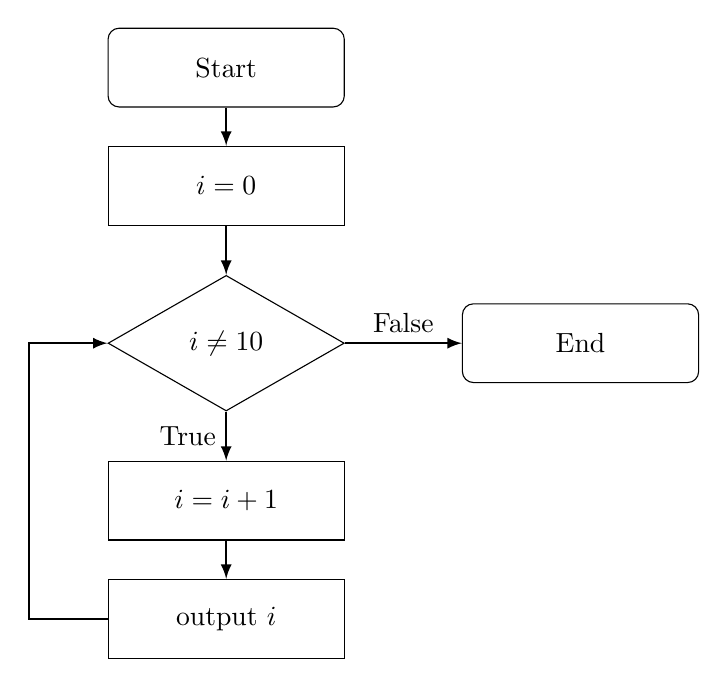
\begin{tikzpicture}[auto, node distance=1.5cm, >=latex]

    % Define styles
    \tikzstyle{startstop} = [rectangle, rounded corners, minimum width=3cm, minimum height=1cm, text centered, draw=black, fill=white]
    \tikzstyle{process} = [rectangle, minimum width=3cm, minimum height=1cm, text centered, draw=black, fill=white]
    \tikzstyle{decision} = [diamond, minimum width=3cm, minimum height=1cm, text centered, draw=black, fill=white]

    % Nodes
    \node (start) [startstop] {Start};
    \node (init) [process, below of=start] {$i = 0$};
    \node (cond) [decision, below of=init, yshift=-0.5cm] {$i \neq 10$};
    \node (inc) [process, below of=cond, yshift=-0.5cm] {$i = i + 1$};
    \node (out) [process, below of=inc] {output $i$};
    \node (end) [startstop, right of=cond, xshift=3cm] {End};

    % Arrows
    \draw [->, thick] (start) -- (init);
    \draw [->, thick] (init) -- (cond);
    \draw [->, thick] (cond) -- node[anchor=east] {True} (inc);
    \draw [->, thick] (inc) -- (out);
    \draw [->, thick] (out.west) -- ++(-1,0) |- (cond.west);
    \draw [->, thick] (cond) -- node[anchor=south] {False} (end);

\end{tikzpicture}
}
    \end{minipage}
    \caption{Algorithm for counting 1 to 10.}
    \label{fig:algorithm}
\end{figure}

We have derived the three corresponding control words for these three data manipulation instructions for controlling the dedicated datapath shown in Figure \ref{fig:datapath}. These three control words are shown here in Figure \ref{fig:control_words}.

\begin{figure}[H]
    \centering
    \resizebox{0.8\textwidth}{!}{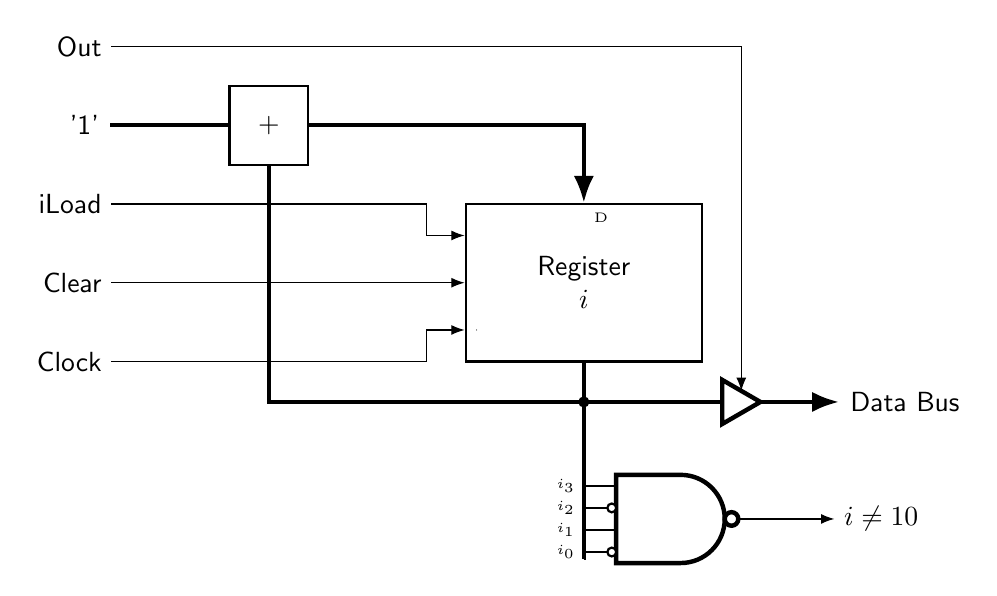
\begin{tikzpicture}[
    font=\sffamily,
    thick,
    >={Latex}
]
    % Use circuitikz IEEE ports
    \ctikzset{logic ports=ieee}

    % Styles for blocks
    \tikzstyle{block} = [draw, rectangle, minimum width=3cm, minimum height=2cm, align=center, fill=white]
    \tikzstyle{adder_style} = [draw, rectangle, minimum width=1cm, minimum height=1cm, align=center, fill=white]

    % Components
    
    % Register i (Center)
    \node [block] (RegI) at (0,0) {Register \\ $i$};

    % Adder (+1) (Top Left - shifted right slightly to make room for control lines if needed, or lines go over/under)
    \node [adder_style] (Adder) at (-4, 2) {+};



    % NAND Gate (Bottom)
    \node [nand port, number inputs=4, scale=1] (Nand) at (1.1, -3) {};
    % Negation bubbles
    \node [left, font=\tiny] at (Nand.in 1) {$i_3$};
    \node [left, font=\tiny] at (Nand.in 2) {$i_2$};
    \node [ocirc,left] at (Nand.bin 2) {}; 
    \node [left, font=\tiny] at (Nand.in 3) {$i_1$};
    \node [left, font=\tiny] at (Nand.in 4) {$i_0$};
    \node [ocirc,left] at (Nand.bin 4) {};

    % Connections

    % 1. Register Output (Bottom) -> Bus Junction
    \draw [line width=1.5pt] (RegI.south) -- ++(0,-0.5) coordinate (bus_junction);
    \node [circ,thick] at (bus_junction) {};

    % Tri-state Buffer (Output) (Right)
    \node [buffer port, scale=0.5] at ($(bus_junction) + (2,0)$) (Buf) {};
    
    % 2. To Buffer (Right)
    \draw [line width=1.5pt] (bus_junction) -- (Buf.bin);
    \draw [->,line width=1.5pt] (Buf.bout) -- ++(1,0) node[right] {Data Bus};

    % 3. To Adder (Left -> Top)
    \draw [line width=1.5pt] (bus_junction)  -| (Adder.south);
    \draw [line width=1.5pt] ($(Adder.west) - (1.5,0)$) node[left] {'1'} -- (Adder.west);
    \draw [->, line width=1.5pt] (Adder.east) -- ++(1,0) -| (RegI.north);
    \node [below right, font=\tiny] at (RegI.north) {D};

    % 4. To NAND (Bottom)
    \draw [line width=1.5pt] (bus_junction) -- ++(0,-2) coordinate (nand_split);
    \draw [thin] (nand_split) -| (Nand.in 1);
    \draw [thin] (nand_split) -| (Nand.in 2);
    \draw [thin] (nand_split) -| (Nand.in 3);
    \draw [thin] (nand_split) -| (Nand.in 4);
    \draw [->, thin] (Nand.out) -- ++(1,0) node[right] {$i \neq 10$};


    % Control Signals - Left Aligned
    % Define start x coordinate for all controls
    \coordinate (ctrl_x) at (-6, 0); 
    
    % iLoad (to Register)
    \draw [thin, ->] (-6, 1) node[left, black] {iLoad} -- (-2, 1) |- ($(RegI.west) + (0, 0.6)$); 
    
    % Clear (to Register)
    \draw [thin, ->] (-6, 0) node[left, black] {Clear} -- (-2, 0) |- (RegI.west); 
    
    % Clock (to Register)
    \draw [thin, ->] (-6, -1) node[left, black] {Clock} -- (-2, -1) |- ($(RegI.west) + (0, -0.6)$);
    % Clock Triangle
    \node [regular polygon, regular polygon sides=3, rotate=-90, inner sep=0pt, scale=0.5, fill=black] at ($(RegI.west) + (0.15, -0.6)$) {};


    \draw [thin, ->] (-6, 3) node[left] {Out} -| (Buf.up);


\end{tikzpicture}
}
    \caption{Dedicated data path for counting 1 to 10.}
    \label{fig:datapath}
\end{figure}

\begin{figure}[H]
    \centering
    
\begin{tabular}{|c|c|c|c|c|}
    \hline
    \textbf{Instruction} & \textbf{Operation} & \textbf{iLoad} & \textbf{Clear} & \textbf{Out} \\
    \hline
    $i = 0$ & Initialize & 0 & 1 & 0 \\
    \hline
    $i = i + 1$ & Increment & 1 & 0 & 0 \\
    \hline
    output $i$ & Output & 0 & 0 & 1 \\
    \hline
\end{tabular}

    \caption{Control words for counting 1 to 10.}
    \label{fig:control_words}
\end{figure}

You are to implement a dedicated datapath for counting 1 to 10.

\begin{enumerate}
    \item Write a VHDL file that defines a datapath using the structured depicted in Figure \ref{fig:datapath}. Your code should include a 4-bit adder, 4-bit register with load and clear, a 4-bit comparator and a quad tri-state buffer. Compile the circuit. How many logic elements (LEs) are used to implement your circuit?
    \item Simulate your circuit to verify its correctness.
    \item Augment your VHDL file to use the pushbutton KEY0 as the Clock input and switches SW2, SW1 and SW0 as iLoad, Clear and Out inputs, LED3 to LED0 to display binary representing the 1 to 10 counts as your circuit operates, and LEDR9 to display the condition ($i \neq 10$). Make the necessary pin assignments needed to implement the circuit on your DE-series board and compile the circuit.
    \item Download your circuit into the FPGA chip and test its functionality by operating the implemented switches.
\end{enumerate}

\section*{Part II}

The state diagram of control unit is derived as shown in Figure \ref{fig:fsm}.

\begin{figure}[H]
    \centering
    
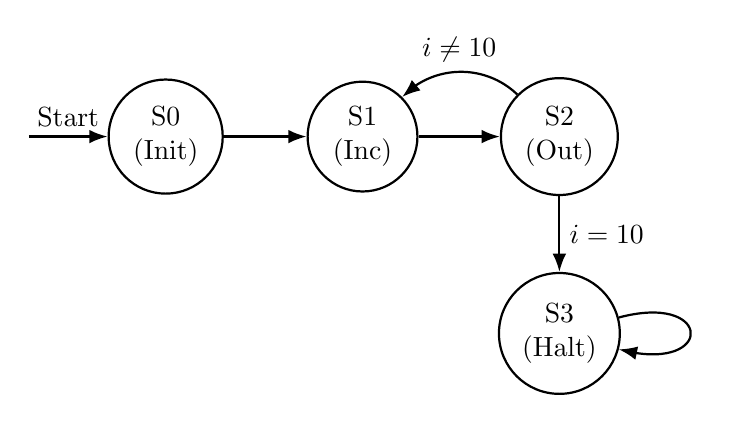
\begin{tikzpicture}[>=Latex, auto, node distance=2.5cm, thick]
    % Define state style locally
    \tikzstyle{state} = [circle, draw, minimum size=1.2cm, align=center]
    
    % States
    \node[state] (S0) {S0\\(Init)};
    \node[state, right of=S0] (S1) {S1\\(Inc)};
    \node[state, right of=S1] (S2) {S2\\(Out)};
    \node[state, below of=S2] (Halt) {S3\\(Halt)};

    % Transitions
    % Start -> S0
    \draw[->] ($(S0.west) + (-1,0)$) -- node[above] {Start} (S0);
    
    % S0 -> S1 (Unconditional)
    \draw[->] (S0) -- (S1);
    
    % S1 -> S2 (Unconditional)
    \draw[->] (S1) -- (S2);
    
    % S2 -> S1 (Loop if i != 10)
    % Bend left?
    \draw[->] (S2) to[bend right=45] node[above] {$i \neq 10$} (S1);
    
    % S2 -> Halt (if i == 10)
    \draw[->] (S2) -- node[right] {$i = 10$} (Halt);
    
    % Halt Self Loop
    \draw[->] (Halt) to[loop right] (Halt);

\end{tikzpicture}

    \caption{State diagram of control unit for counting 1 to 10.}
    \label{fig:fsm}
\end{figure}

You are to implement a control unit that cooperate with the dedicated datapath.

\begin{enumerate}
    \item Write a VHDL file that defines a finite state machine (FSM) depicted in Figure \ref{fig:fsm}. Your code should include a state variable that hold the current state (s0...s3), a reset input to initialize the state to s0 and the control signals (iLoad, Clear and Out) as outputs to the datapath. Compile the circuit. How many logic elements (LEs) are used to implement your circuit?
    \item Simulate your circuit to verify its correctness.
    \item Augment your VHDL file to use the pushbutton KEY0 as the Clock input and switches SW1 and SW0 as Reset and ($i \neq 10$) inputs, and three LEDR2-0 to display iLoad, Clear and Out as your circuit operates. Make the necessary pin assignments needed to implement the circuit on your DE-series board and compile the circuit.
    \item Download your circuit into the FPGA chip and test its functionality by operating the implemented switches.
\end{enumerate}

\section*{Part III}

The dedicated microprocessor consisting of a Control unit and a Datapath shown in Figure \ref{fig:microprocessor}.

\begin{figure}[H]
    \centering
    \resizebox{\textwidth}{!}{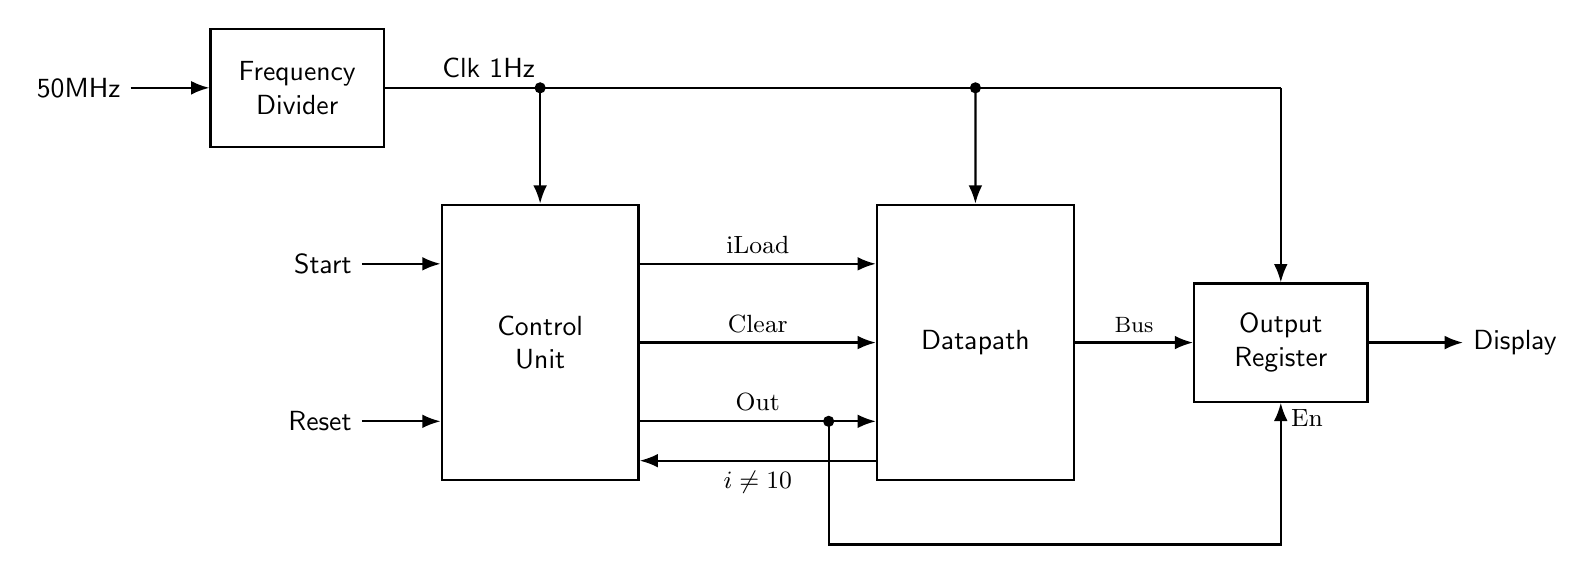
\begin{tikzpicture}[
    font=\sffamily,
    >=Latex,
    thick,
    block/.style={draw, rectangle, minimum width=2.5cm, minimum height=3.5cm, align=center, fill=white},
    sblock/.style={draw, rectangle, minimum width=2.2cm, minimum height=1.5cm, align=center, fill=white}, 
    signal/.style={->}
]

    % Components
    \node [block] (Control) at (0,0) {Control\\Unit};
    \node [block, right=3cm of Control] (Datapath) {Datapath};
    \node [sblock, above left=1cm of Control] (FreqDiv) {Frequency\\Divider};
    \node [sblock, right=1.5cm of Datapath] (OutReg) {Output\\Register};

    % 1. Clock System
    % Input 50MHz to FreqDiv
    \draw [signal] ($(FreqDiv.west) + (-1, 0)$) node[left] {50MHz} -- (FreqDiv.west);
    
    % System Clock distribution
    % Run a bus along the top
    \coordinate (clk_bus_y) at (2.5, 2.5); % High above blocks (y=1.75 is top)
    \draw [-] (FreqDiv.east) -- ++(0.2, 0) coordinate (clk_bus_start); % Up to y=~2.0
    \draw [-] (clk_bus_start) -- (OutReg|-clk_bus_start) coordinate (clk_bus_end);
    \node [above] at ($(clk_bus_start)!0.1!(clk_bus_end)$) {Clk 1Hz};

    % Drop downs
    \draw [signal] (Control|-clk_bus_start) to[short,*-] (Control.north);
    \draw [signal] (Datapath|-clk_bus_start) to[short,*-] (Datapath.north);
    \draw [signal] (OutReg|-clk_bus_start) -- (OutReg.north);

    % 2. External Inputs (Control)
    \draw [signal] ($(Control.west) + (-1, 1)$) node[left] {Start} -- ($(Control.west) + (0, 1)$);
    \draw [signal] ($(Control.west) + (-1, -1)$) node[left] {Reset} -- ($(Control.west) + (0, -1)$);

    % 3. Control Signals (Control -> Datapath)
    \draw [signal] ($(Control.east) + (0, 1)$) -- node[above, font=\small] {iLoad} ($(Datapath.west) + (0, 1)$);
    \draw [signal] ($(Control.east) + (0, 0)$) -- node[above, font=\small] {Clear} ($(Datapath.west) + (0, 0)$);
    
    % Out Signal & Overlap Fix
    % Out comes from Control y=-1.
    % Route to Datapath straight.
    \draw [signal] ($(Control.east) + (0, -1)$) -- node[above, font=\small] {Out} coordinate[pos=0.8] (out_tap) ($(Datapath.west) + (0, -1)$);
    
    % Tap to OutReg En
    % Go DOWN deep to avoid i!=10
    \draw node[circ] at (out_tap) {};
    \draw [->] (out_tap) |- ($(Datapath.south) + (0, -0.8)$) -| (OutReg.south);
    \node [right, font=\small, yshift=-0.2cm] at (OutReg.south) {En};

    % 4. Status Signal (Datapath -> Control)
    % i != 10
    % Route slightly lower than straight to differentiate, but above the Out bypass
    \draw [signal] ($(Datapath.west) + (0, -1.5)$) -- node[below, font=\small] {$i \neq 10$} ($(Control.east) + (0, -1.5)$);
    
    % 5. Data Flow
    \draw [signal] ($(Datapath.east) + (0, 0)$) -- node[above, font=\footnotesize] {Bus} (OutReg.west);
    \draw [signal] (OutReg.east) -- ++(1.2, 0) node[right] {Display};

\end{tikzpicture}
}
    \caption{Dedicated microprocessor for counting 1 to 10.}
    \label{fig:microprocessor}
\end{figure}

You are to implement a dedicated microprocessor by assembling the Control unit and Datapath.

\begin{enumerate}
    \item Write a VHDL file that defines component circuit (created in Part I and Part II), depicted in Figure \ref{fig:microprocessor}. Modify the control unit to be able to operate with system internal clock (use a counter to transform 50 MHz to 1 Hz trigger or clock signal with period of 1 second). Compile the circuit. How many logic elements (LEs) are used to implement your circuit?
    \item Simulate your circuit to verify its correctness.
    \item Augment your VHDL file to use a pushbutton KEY0 as Reset, and a 7-segment display HEX0 to display the 1 to 10 (‘A’) count as your circuit operates. Note that the datapath output bus is tri-stated. To drive the 7-segment display correctly, you must capture the output value when the `Out` signal is active. Instantiate an intermediate register (enabled by `Out`) between the datapath bus and the 7-segment decoder to hold the value when the bus is in the high-impedance state. Make the necessary pin assignments needed to implement the circuit on your DE-series board and compile the circuit.
    \item Download your circuit into the FPGA chip and test its functionality by operating the implemented switches.
    \item What is the frequency of the display updates? What to modify if you want to make it changes exactly 1 Hz?
\end{enumerate}

\vspace{1cm}
\noindent \textbf{Updated By:} R. Sutthaweekul \\
\textbf{Release Date:} 2026-01-02

\end{document}
